\documentclass[12pt,oneside,openany,letterpaper]{article}


\usepackage{fancyhdr}
\usepackage{helvet}
\usepackage{amsmath}
%\usepackage{graphicx}
\usepackage{psfrag}
\usepackage{setspace}
%\usepackage[hypertex, linktocpage]{hyperref}[2003/11/30]
\usepackage[linktocpage]{hyperref}[2003/11/30]
\usepackage{lscape}
\usepackage{nicefrac}
\usepackage{mathrsfs}
\usepackage{units}
\usepackage{upgreek}
\usepackage{amssymb}
\usepackage{color}
\usepackage{wrapfig}
\usepackage{multirow}
\usepackage{url}
\usepackage{verbatim}
\usepackage[pdftex]{graphicx}
\usepackage{epstopdf}
\usepackage{enumitem}


\onehalfspacing \setlength\textheight{667pt}
\setlength\textwidth{506pt} \setlength\oddsidemargin{-18pt}
\setlength\topmargin{-20pt}
%\setlength\footskip{24pt}
\addtolength\headheight{2.5pt} \addtolength\headsep{-14pt}
%\fancyhead[R]{\includegraphics[height=10.5pt]{ubclogo_bw.eps}\#:  55907968}
%\renewcommand\familydefault{\sfdefault}


%\fancyhead[L]{Name:} \fancyhead[R]{Student
%Number:~~~~~~~~~~~~~~~~~~~~~~~~~~~~~~~~~~~~~~~~~~}
\fancyhead[L]{\emph{Introduction to Electronics}}\fancyhead[R]{Operational Amplifiers}
\fancyfoot[L]{PHYS 231}\fancyfoot[R]{Experiment 5}
\pagestyle{fancy} \pagenumbering{arabic}


\newenvironment{packed_enum}{
\begin{enumerate}
  \setlength{\itemsep}{0pt}
  \setlength{\parskip}{0pt}
  \setlength{\parsep}{0pt}
}{\end{enumerate}}


\newenvironment{packed_item}{
\begin{itemize}
  \setlength{\itemsep}{0pt}
  \setlength{\parskip}{0pt}
  \setlength{\parsep}{0pt}
}{\end{itemize}}


\begin{document}

\thispagestyle{plain}
\begin{center}
{\large{\bf{\fontfamily{phv}\selectfont Physics 231 - Operational Amplifiers (Exp.~5)}}}
\end{center}

\noindent GOALS AND SUMMARY

~

\noindent Operational amplifiers (op amps) are very versatile devices used in a wide variety of applications. Some of the basic properties of op amps will be investigated in this lab, with an emphasis on practicality. Common problems and limitations will be outlined. 

~

\noindent INTRODUCTION

~

\noindent Modern technology has virtually eliminated the necessity of a user to construct amplifiers from discrete components. There are very few amplifier applications for which the experimenter cannot purchase a small inexpensive unit to perform the required task. These inexpensive circuits are themselves very complex, integrated circuits, the most common of which is the op amp.

~

\noindent TERMS AND JARGON:

~
 
\noindent The op amp symbol is shown in Fig.~\ref{fig:1}.  The pin designations shown apply to the LM741 op amp that you will use in this experiment.
\begin{figure}[h!]
\begin{center}
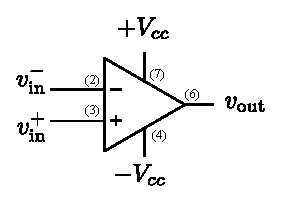
\includegraphics[width=5.5 cm]{opamp.eps}
\caption{\label{fig:1}The LM741 op amp pin designations. $+V_\mathrm{cc}=15$~V and $-V_\mathrm{cc}=-15$~V are the positive and negative supply voltage that you must provide the op amp.  The inverting input is $v_\mathrm{in}^-$, the non-inverting input is $v_\mathrm{in}^+$, and the output is $v_\mathrm{out}$.}
\end{center}
\end{figure}

~

\noindent In circuit diagrams, the power supply lines $(\pm V_\mathrm{cc})$ are usually omitted, so always be sure to {\bf connect the dc power} (usually $+15$ and $-15\rm\ V$) even if it is not indicated on the circuit diagram. 

\clearpage

The following terms are frequently encountered when dealing with op amp circuits:
\begin{itemize}
\item Voltage gain $(G)$:  The output voltage of the circuit containing the op amp divided by the input voltage.  The voltage gain of the op amp unit, ITSELF, is usually referred to as the open-loop voltage gain $(A_\mathrm{OL})$ of the op amp. 
\item Input impedance: The effective resistance between the inputs $v_\mathrm{in}^-$ (pin 2) and $v_\mathrm{in}^+$ (pin 3).  Op amps are designed to have a VERY large input impedance. 
\item Output resistance: The effective resistance in series with $v_\mathrm{out}$ (pin 6).  Op amps are designed to have a low output resistance. 
\item	Bandwidth: The frequency range over which the gain $G$ is nearly constant. 
\end{itemize}

~

{\bf THE NON-IDEAL CHARACTERISTICS OF OP AMPS TO BE AWARE OF:}
\begin{itemize}
\item The amplifier draws a minute amount of current ($\sim 100$~nA) through its inputs at all times.  This is called the ``{\bf input offset current}".  The amplifier is also characterized by a slight, D.C. ``{\bf input offset voltage}" ($\sim 1$~mV). 
\item The gain of the amplifier decreases with increasing frequency. This is a deliberate design characteristic, which reduces the tendency of the amplifier to oscillate. 
\item The value of the output voltage signal can never exceed the supply voltages $(\pm V_\mathrm{cc})$.
\end{itemize}

~

\noindent THE INVERTING AMPLIFIER

~

\noindent A simple, but practical, amplifier is shown in Fig.~\ref{fig:2}.
\begin{figure}[h!]
\begin{center}
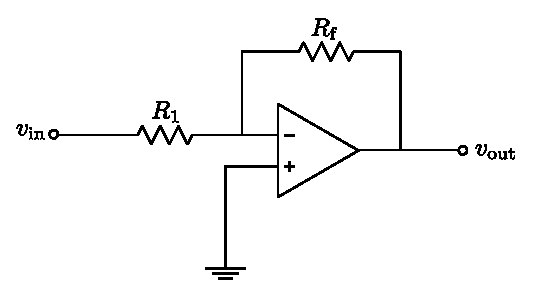
\includegraphics[width=9.5 cm]{inverting.eps}
\caption{\label{fig:2}The inverting amplifier.}
\end{center}
\end{figure}
Its voltage gain, $G$, is given by:
\begin{equation}
G=\frac{v_\mathrm{out}}{v_\mathrm{in}}=-\frac{R_\mathrm{f}}{R_1}
\end{equation}
This is the ideal behaviour of the circuit as a linear amplifier (i.e. the output voltage is linearly proportional to the input voltage). However, there are several restrictions on this ideal behaviour (and you'll explore some of these as you do this experiment).

~

{\bf Restrictions}

~

\begin{tabular}{rp{12.5 cm}}
$\vert v_\mathrm{in}\vert > 10$~mV & Required such that the input noise, the input offset current, and the input offset voltage do not interfere with the measurements at the output.\\
~ & ~\\
$\vert G\cdot v_\mathrm{in}\vert<V_\mathrm{sat}\approx 14~V$ & Required to ensure that $v_\mathrm{out}$ is not asked to output a voltage that is greater than that provided by the power supply.\\
~ & ~\\
$f\cdot G<10^5$ & Where $f$ is the maximum frequency to be amplified.  This gain-bandwidth product is determined by the natural bandwidth and open-loop gain of the op amp.
\end{tabular}

~

\noindent EXPERIMENT

~

\noindent Construct the inverting amplifier circuit shown in Fig.~\ref{fig:2} on the circuit board provided, using $R_1=1~\mathrm{k}\Omega$ for the input resistor and $R_\mathrm{f} = 100~\mathrm{k}\Omega$ for the feedback resistor. The pin diagrams and details on the 741 op amp can be found on the course website.  

~

\noindent First, use a small amplitude sine wave for the input voltage. Try varying the amplitude of the sine wave. You will find that an input amplitude that is too large can easily cause the amplifier to saturate, giving a distorted or ``clipped" waveform.  At what positive and negative output voltages does the signal get clipped? During your work with op amps you should always be wary of such distortions and you may find that you need to adjust the amplitude of the generator if the output of the amplifier is saturating.

~

\noindent In addition to this problem, there are more subtle distortions that can occur. You can see some of these by increasing the frequency of the generator high enough that the output amplitude from the amplifier decreases drastically. Then qualitatively investigate what happens when you vary the amplitude of the input signal. You are likely to see a distorted waveform of some sort and non-linear behaviour (meaning that the output amplitude no longer varies linearly with the input amplitude). These potential problems should be kept in mind when making the remainder of the measurements.

~

\noindent Now, over a wide frequency range, measure the gain $G$ of the output voltage relative to the input voltage. Determine the bandwidth $BW$ of the amplifier by finding the frequency at which the gain drops to $1/\sqrt{2}$ of the gain at low frequencies (always making sure that you are working in the linear regime of the amplifier). A Jupyter notebook will be used to plot $\log\left\vert G\right\vert$ as a function of $\log f$.  You will also perform a linear fit to determine the power law that governs the roll-off above this cutoff frequency.

~

\noindent Next, explore a wide range of gains and bandwidths by using several different combinations of resistors for $R_1$ and $R_\mathrm{f}$. For each case measure the low-frequency gain $G$ and the bandwidth $BW$. You should do this quickly: for each combination of resistors, measure the low-frequency gain and then increase the frequency until the gain drops to $1/\sqrt{2}$ of the low-frequency value. Make a plot of the bandwidth versus the gain.


\end{document}
